\section{Residual dynamics and the centring identity}
\label{sec:residual}

\subsection{Transform and regime structure}

Electricity prices are bounded below by an administrative floor, occasionally
negative in other markets \citep{AustHorsch2020}, and heavy-tailed above. The
underlying estimation exercise works on the inverse hyperbolic sine transform,
\begin{equation}
  y_t = \operatorname{asinh}\!\left(\frac{P_t}{s_P}\right),
  \qquad
  P_t = s_P \sinh(y_t),
  \label{eq:asinh}
\end{equation}
with scale $s_P = 282.48$ \TRY. The transform is odd, defined on the whole real
line and asymptotically logarithmic, so it compresses spikes without the
domain restriction of a log transform.

Let $S_t\in\{0,1\}$ be a continuous-time Markov chain, with state $0$ the calm
regime and state $1$ the stress regime, distinguished by their diffusion
coefficients $\sigma^y_0 \ll \sigma^y_1$. Regime volatilities are inherited
from the underlying estimation as $\sigma^y_0 = 0.003535$ and
$\sigma^y_1 = 0.092407$ per $\sqrt{\text{hour}}$, a ratio of roughly $26$.

\subsection{Time-varying transition probabilities}

Transition probabilities depend on standardised residual demand at a one-hour
lag through a logistic link,
\begin{equation}
  p_{01}(t) = \Lambda\!\left(\alpha_{01}+\gamma_{01} z_{t-1}\right),
  \qquad
  p_{10}(t) = \Lambda\!\left(\alpha_{10}+\gamma_{10} z_{t-1}\right),
  \qquad
  \Lambda(x)=\frac{1}{1+e^{-x}},
  \label{eq:tvtp}
\end{equation}
following \citet{Diebold1994} and \citet{Filardo1994}; consistency of maximum
likelihood estimation for this class with covariate-dependent transitions is
established by \citet{Pouzo2022}, and \citet{Bazzi2017} develop the
score-driven alternative. The lag structure matters for interpretation:
$z_{t-1}$ is the residual demand observed \emph{before} the transition it
governs, so the specification is predictive rather than contemporaneous.

Figure~\ref{fig:tvtp} shows the two fitted transition functions against the
sample distribution of the covariate. Over the bulk of the sample the calm-to-stress
probability exceeds the reverse, and the two cross near $z\approx 1.4$; the
economic reading of that crossing is deferred to Section~\ref{sec:sensitivity},
where the covariate channel is quantified.

\begin{figure}[htbp]
\centering
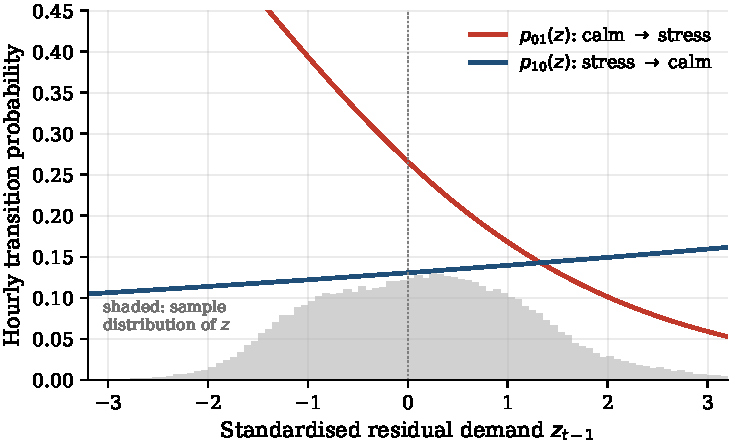
\includegraphics[width=\textwidth]{figures/tvtp_mechanism.pdf}
\caption{Fitted hourly transition probabilities against standardised residual
demand, with the sample distribution of the covariate shaded.}
\label{fig:tvtp}
\end{figure}

The discrete one-step probabilities \eqref{eq:tvtp} are converted to
continuous-time intensities by matrix logarithm. For the two-state chain with
one-step matrix
$\Pi(t) = \begin{psmallmatrix} 1-p_{01} & p_{01}\\ p_{10} & 1-p_{10}\end{psmallmatrix}$
and $s = p_{01}+p_{10}$, the generator is
\begin{equation}
  Q(t) =
  \begin{bmatrix} -q_{01}(t) & q_{01}(t)\\ q_{10}(t) & -q_{10}(t)\end{bmatrix},
  \qquad
  q_{0 1}(t) = \frac{\lambda(t)\,p_{01}(t)}{s(t)},
  \quad
  \lambda(t) = -\ln\!\left(1-s(t)\right),
  \label{eq:generator}
\end{equation}
with $q_{10}$ defined symmetrically, reducing to $q_{ij}\approx p_{ij}/\Delta t$
when $s$ is small. The embedding is exact whenever $s<1$, which holds
throughout our sample. Appendix~\ref{app:transitions} documents the regime
label reconciliation this conversion required.

\subsection{Residual process and price-space diffusion}

Conditional on the regime, the residual follows an Ornstein--Uhlenbeck process
in price space,
\begin{equation}
  \dif X_t = \kappa\left(m_{S_t} - X_t\right)\dif t
             + \sigma^X_{S_t}(t)\,\dif W_t,
  \label{eq:ou}
\end{equation}
with a common mean-reversion rate $\kappa$ and regime-dependent targets $m_i$.
The diffusion coefficient is mapped from transform space to price space by the
delta method applied to \eqref{eq:asinh}. Since
$\dif P/\dif y = \sqrt{P^2+s_P^2}$, evaluating at the forward level gives
\begin{equation}
  \sigma^X_i(t) = \sigma^y_i\,\sqrt{F(t)^2 + s_P^2}\,,
  \label{eq:sigmamap}
\end{equation}
which is state-dependent through $F$ and therefore time-varying even for fixed
$\sigma^y_i$. At $F\approx 2{,}900$ \TRY{} the factor is approximately
$2{,}914$, so the stress-regime price-space diffusion is on the order of
$269$ \TRY{} per $\sqrt{\text{hour}}$.

Two properties of \eqref{eq:ou} deserve emphasis. It is additive rather than
multiplicative, so the model can in principle generate negative terminal
prices; we report the simulated probability of that event in
Section~\ref{sec:results} and treat it as a diagnostic of specification
adequacy. And $\kappa$ is shared across regimes, so regime switching enters the
second moment but not the speed of mean reversion, which keeps the moment
system linear.

\subsection{Forward centring}

The spot price is defined as
\begin{equation}
  \boxed{\;P_t \;=\; F(t) \;+\; X_t \;-\; \mu_X(t),
  \qquad \mu_X(t) \;=\; \E^{\Q}\!\left[X_t\right].\;}
  \label{eq:centering}
\end{equation}

\begin{proposition}[Exact first-moment anchoring]
\label{prop:centering}
Let $X$ satisfy \eqref{eq:ou} with regime process generated by \eqref{eq:generator},
let $\mu_X(t)=\E^{\Q}[X_t]$ be computed under the same measure and the same
parameters used in \eqref{eq:centering}, and let $P$ be defined by
\eqref{eq:centering}. Then
\begin{equation*}
\begin{gathered}
  \E^{\Q}\!\left[P_t\right] = F(t)
  \quad\text{for all } t, \text{ and for every admissible}\\[2pt]
  \left(\kappa,\ \sigma^y_0,\ \sigma^y_1,\ m_0,\ m_1,\
        \alpha_{01},\ \alpha_{10},\ \gamma_{01},\ \gamma_{10},\ \pi_0\right).
\end{gathered}
\end{equation*}
\end{proposition}

\begin{proof}
Taking expectations in \eqref{eq:centering} and using linearity,
$\E^{\Q}[P_t] = F(t) + \E^{\Q}[X_t] - \mu_X(t) = F(t) + \mu_X(t) - \mu_X(t)
= F(t)$. The content of the statement is not the algebra but the requirement
that $\mu_X$ be the \emph{same} functional of the parameters that drives the
dynamics, evaluated by the same numerical procedure. Section~\ref{sec:moments}
shows that $\mu_X(t)=u_0(t)+u_1(t)$, where $u_i$ solve the coupled first-moment
system \eqref{eq:momentsys}. Since that system is integrated jointly with the
regime probabilities used in pricing, the cancellation is exact in
floating-point arithmetic up to integration tolerance, rather than approximate.
\end{proof}

\begin{remark}
Proposition~\ref{prop:centering} is what permits the identification argument of
this paper. Whatever is wrong with the inherited regime parameters, and
Section~\ref{sec:results} shows that a great deal was wrong with one of them,
none of it can corrupt the first moment. Errors in the residual layer are
confined to the shape of the distribution around a forward level that remains
pinned to observed quotes.
\end{remark}

\begin{remark}[Contrast with a multiplicative specification]\label{rem:multiplicative}
An earlier specification of this project modelled the price directly as
$P_t = s_P\sinh(Y_t)$ with $Y$ a regime-switching OU process, for which
$\E[P_t] = s_P e^{v(t)/2}\sinh(m(t))$ with $v$ the transform-space variance.
This form fails to anchor to the forward in two distinct ways depending on the
mean-reversion rate. Under a near-unit-root $\kappa$ the variance $v$ grows
almost linearly in horizon and the factor $e^{v/2}$ inflates the implied
forward without bound. Under the corrected $\kappa$ of
Section~\ref{sec:provenance} the inflation is mild, reaching only $1.019$ at
its stationary value, but the regime-weighted mean $m(t)$ is negative, so the
implied expected spot converges to approximately $-3{,}108$ \TRY{} against an
observed forward of $+2{,}916$ \TRY. Neither failure is a parameter problem
that better estimation would fix; both follow from letting the residual
dynamics determine the implied forward. The additive centred form removes the
question by construction, which was the original motivation for adopting it.
We retain the comparison in Section~\ref{sec:results} because it quantifies
what the centring buys.
\end{remark}
